\documentclass[cjk,slidestop,handout,compress,mathserif,blue]{beamer}	%打印PPT用,handout(讲义)可去掉过渡效果,如\pause引起的多页显示,为打印时节省纸张
%dvipdfm选项是关键,否则编译统统通不过
%beamer的颜色选项定义的是导航条和标题的颜色(即关键词structure的颜色)

%%%%%%%%%%%%%%%%仅限于XeTeX可使用的宏包%%%%%%%%%%%%%%%%%%%%%%%%%%%%
\usepackage{fontspec,xunicode,xltxtra,beamerthemesplit}
%\usepackage{beamerthemesplit}
\usepackage{xeCJK}
\setCJKmainfont[BoldFont=黑体, ItalicFont=楷体, BoldItalicFont=仿宋]{黑体}
%\setsansfont[Mapping=tex-text]{Adobe 黑体 Std}
%如果装了Adobe Acrobat,可在font.conf中配置Adobe字体的路径以使用其中文字体
%也可直接使用系统中的中文字体如SimSun,SimHei,微软雅黑 等
%原来beamer用的字体是sans family;注意Mapping的大小写,不能写错

%%%%%%%%   确定标题和导航条结构的框架     %%%%%%%%%%%%
\usepackage{beamerthemeshadow}                       %
%\usepackage{beamerthemeclassic}%导航条色与背景色一致%
%%%%%%%%%%%%%%%%%%%%%%%%%%%%%%%%%%%%%%%%%%%%%%%%%%%%%%
\setbeamerfont{roman title}{size={}}
%\usepackage{CJK} % CJK 中文支持                                  %
\usepackage{amsmath,amsthm,amsfonts,amssymb,bm}
\usepackage{mathrsfs}
\usepackage{xcolor}                                        %使用默认允许使用颜色
\usepackage{hyperref} 
\usepackage{graphicx}
\usepackage{subfigure}           %图片跨页

%\usepackage[numbers,sort&compress]{natbib} %紧密排列             %
\usepackage[sectionbib]{chapterbib}        %每章节单独参考文献   %
\usepackage{hypernat}                                                                         %
%\usepackage[dvipdfm,bookmarksopen=true,pdfstartview=FitH,CJKbookmarks]{hyperref}		%
\hypersetup{bookmarksnumbered,colorlinks,linkcolor=brown,citecolor=blue,urlcolor=red}         %
%参考文献含有超链接引用时需要下列宏包,注意与natbib有冲突        %
%\usepackage[dvipdfm]{hyperref}                                  %
%\usepackage{hypernat}                                           %
\newcommand{\upcite}[1]{\hspace{0ex}\textsuperscript{\cite{#1}}} %

%\useoutertheme{smoothbars}
\useinnertheme[shadow=true]{rounded}
\usetheme{Berkeley}                                          %主题式样
%\usetheme{Luebeck}

\usecolortheme{lily}                                        %颜色主题式样

\usefonttheme{professionalfonts}                           %字体主题样式宏包

%\beamertemplatetransparentcoveredhigh                      %使所有被隐藏的文本高度透明
\beamertemplatetransparentcovereddynamicmedium             %使所有被隐藏的文本完全透明,动态,动态的范围很小
\mode<presentation>
%\beamersetaveragebackground{gray}                          %设置背景颜色(单一色) 
\beamertemplateshadingbackground{green!10}{red!5}         %设置背景颜色(渐变色)

%在指定位置精确放置logo
\usepackage{tikz}
\usepackage{beamerfoils}
\usepackage{pgf}
\logo{\pgfputat{\pgfxy(11.68,0.15)}{\includegraphics[height=1.01cm,viewport=0 0 140 120,clip]{Figures/BCC_logo-1.png}}\pgfputat{\pgfxy(10.502,-0.218)}{\includegraphics[height=0.369cm,viewport=140 0 540 120,clip]{Figures/BCC_logo-1.png}}}
%\logo{\pgfputat{\pgfxy(11.68,0.15)}{\includegraphics[height=0.95cm,viewport=0 0 510 360,clip]{Figures/Logo_Gainstrong.png}}\pgfputat{\pgfxy(10.333,-0.195)}{\includegraphics[height=0.35cm,viewport=530 70 1100 218,clip]{Figures/Logo_Gainstrong.png}}}
%\MyLogo{
%	\pgfputat{\pgfxy(-50,-50)}{\pgfbox[right,base]{\includegraphics[height=1cm]{Figures/BCC_logo-1.png}}}
%logo作为背景放置
%\setbeamertemplate{background}{
%	\pgfputat{\pgfxy(6.5,-0.5)}{\pgfbox[left,top]{\pgfimage[height=1.1cm]{Figures/BCC_logo-1.png}}}}

%\logo{}									%不显示logo

\begin{document}
%\begin{CJK*}{GBK}{song}
%\begin{CJK*}{GBK}{kai}
%beamer下不能用\songyi、\zihao等命令!
%\graphicspath{Figures/}

%-------------------------------PPT Title-------------------------------------
\title{课题任务年度进展}
%-----------------------------------------------------------------------------

%----------------------------Author & Date------------------------------------
%\author[Jiang]{姜\;\;骏\inst{}} %[]{} (optional, use only with lots of authors)
% - Give the names in the same order as the appear in the paper.
% - Use the \inst{?} command only if the authors have different
%   affiliation.
\institute[BCC]{\inst{}%
 \vskip -5pt 北京市计算中心}
\date[\today] % (optional, should be abbreviation of conference name)
{
%{\fontsize{6.2pt}{3.2pt}\selectfont{\textcolor{blue}{E-mail:~}\url{jiangjun@bcc.ac.cn}}}
%\vskip 30pt {\fontsize{6.2pt}{3.2pt}\selectfont{清华大学\;\;物理系}}
%\vskip 35pt {\fontsize{8.2pt}{6.2pt}\selectfont{上海}}
%\vskip 5pt {\fontsize{7.2pt}{3.2pt}\selectfont{2019.~06}}
}

% - Either use conference name or its abbreviation
% - Not really information to the audience, more for people (including
%   yourself) who are reading the slides online

\subject{TEST-2}
% This is only inserted into the PDF information catalog. Can be left
% out.
\frame
{
%	\frametitle{\fontsize{9.5pt}{5.2pt}\selectfont{\textcolor{orange}{“高通量并发式材料计算算法与软件”中期检查}}}
	\frametitle{\fontsize{9.5pt}{5.2pt}\selectfont{\textcolor{orange}{“高通量并发式材料计算算法与软件”专题讨论}}}
\titlepage
}
%-----------------------------------------------------------------------------

%------------------------------------------------------------------------------列出全文 outline ---------------------------------------------------------------------------------
\section*{}
\frame[allowframebreaks]
{
  \frametitle{Outline}
%  \frametitle{\textcolor{mycolor}{\secname}}
  \tableofcontents%[current,currentsection,currentsubsection]
}
%在每个section之前列出全部Outline
%类似的在每个subsection之前列出全部Outline是\AtBeginSubsection[]
\AtBeginSection[]
{
  \frame<handout:0>
  {
    \frametitle{Outline}
%全部Outline中,本部分加亮
    \tableofcontents[current,currentsection]
  }
}

%------------------------------------------------------------------------------PPT main Body------------------------------------------------------------------------------------
\small
\section{空间群对称性分析模块与$\vec k$-\rm{path~}路径}
\frame
{
	\frametitle{传统能带计算的问题}
	初基原胞相同的材料电子结构表现出一定的相似性,但传统能带计算和表示的$\vec k$点路径($\vec k$-\textrm{Path})选择有着明显的人为性和任意性
%\vspace{10pt}
\begin{figure}[h!]
\centering
\hspace*{-0.30in}
\subfigure[\fontsize{6.5pt}{5.2pt}\selectfont{\textrm{Brillouin Zone of BCC lattice}}]{
\label{Brillouin_Zone_BCC}
\includegraphics[height=1.5in,width=1.6in,viewport=00 0 550 520,clip]{Figures/Brillouin-Zone_BCC.png}}
%\vskip 0.10in
\subfigure[\textrm{Band structure of GeF$_4$}]{
\label{Band_Gap_GeF4}
\includegraphics[height=1.05in,width=1.65in,viewport=0 0 750 500,clip]{Figures/Band-Struct_GeF4.png}}
\label{Band_Gap_BCC_GeF4}
\end{figure}
利用对称性模块实现\textcolor{red}{能带表示路径~$\vec k$-\textrm{path}“标准化”},对于高通量材料电子结构数据挖掘有着重要意义\upcite{CMS49-299_2010}
}

%\frame
%{
%	\frametitle{标准化的对称性模块}
%\begin{enumerate}
%   \setlength{\itemsep}{20pt}
%	\item 结构文件转换子模块:~\textcolor{magenta}{不同格式的结构文件间的相互转换}
%	\item 对称性分析功能子模块
%		\begin{itemize}
%			\item 确定原胞的点群、空间群和对称操作矩阵
%			\item 标准化的初基原胞(\textrm{primitive cell})
%				\vskip 2pt
%				\textcolor{magenta}{按晶轴长度和晶面夹角的大小确定晶格矢量排列顺序}
%		\end{itemize}
%	\item 标准化$\vec k$~点生成子模块\upcite{CMS49-299_2010}
%		\begin{itemize}
%			\item 确定14种\textrm{Bravais~}格子所有标准化\textrm{Wigner-Seitz~}原胞
%			\item 确定所有高对称性点的分数坐标和能带图中$\vec k$-\textrm{path}
%		\end{itemize}
%	\item 标准化结构参数的数据存储:~\textcolor{magenta}{元素、晶格、对称性等信息}
%\end{enumerate}
%}

%\frame
%{
%	\frametitle{标准化结构参数的数据存储子模块}
%\begin{figure}[h!]
%\centering
%\vspace*{-0.2in}
%\includegraphics[height=2.5in,width=3.7in,viewport=0 0 850 540,clip]{Figures/MP_database_structure.png}
%\caption{\fontsize{7.2pt}{4.2pt}\selectfont{\textrm{Basic database schema for storing periodic crystal structures. Ref\cite{CMS50-2295_2011}}}}%
%\label{MP_structure_data}
%\end{figure} 
%}
%
\frame
{
	\frametitle{\textrm{VASP~}点群对称性判断与晶胞选择}
	在\textrm{VASP~}中,对应的对称性判断为
\begin{figure}[h!]
\centering
\vspace*{-0.1in}
\hspace*{-0.15in}
\includegraphics[height=2.3in,width=4.3in,viewport=0 0 1080 530,clip]{Figures/VASP_FCC_Si_symmetry.png}
%\caption{\fontsize{7.2pt}{4.2pt}\selectfont{\textrm{Basic database schema for storing periodic crystal structures. Ref\cite{CMS50-2295_2011}}}}%
\label{FCC_Si-OUTCAR}
\end{figure} 
}

%\frame
%{
%	\frametitle{\textrm{VASP~}软件的对称性判断与能带绘制}
%	根据\textrm{VASP~}计算得到\textrm{FCC-Si}的电子结构:\textrm{DOS}
%\begin{figure}[h!]
%\centering
%\vspace*{-0.1in}
%\hspace*{-0.20in}
%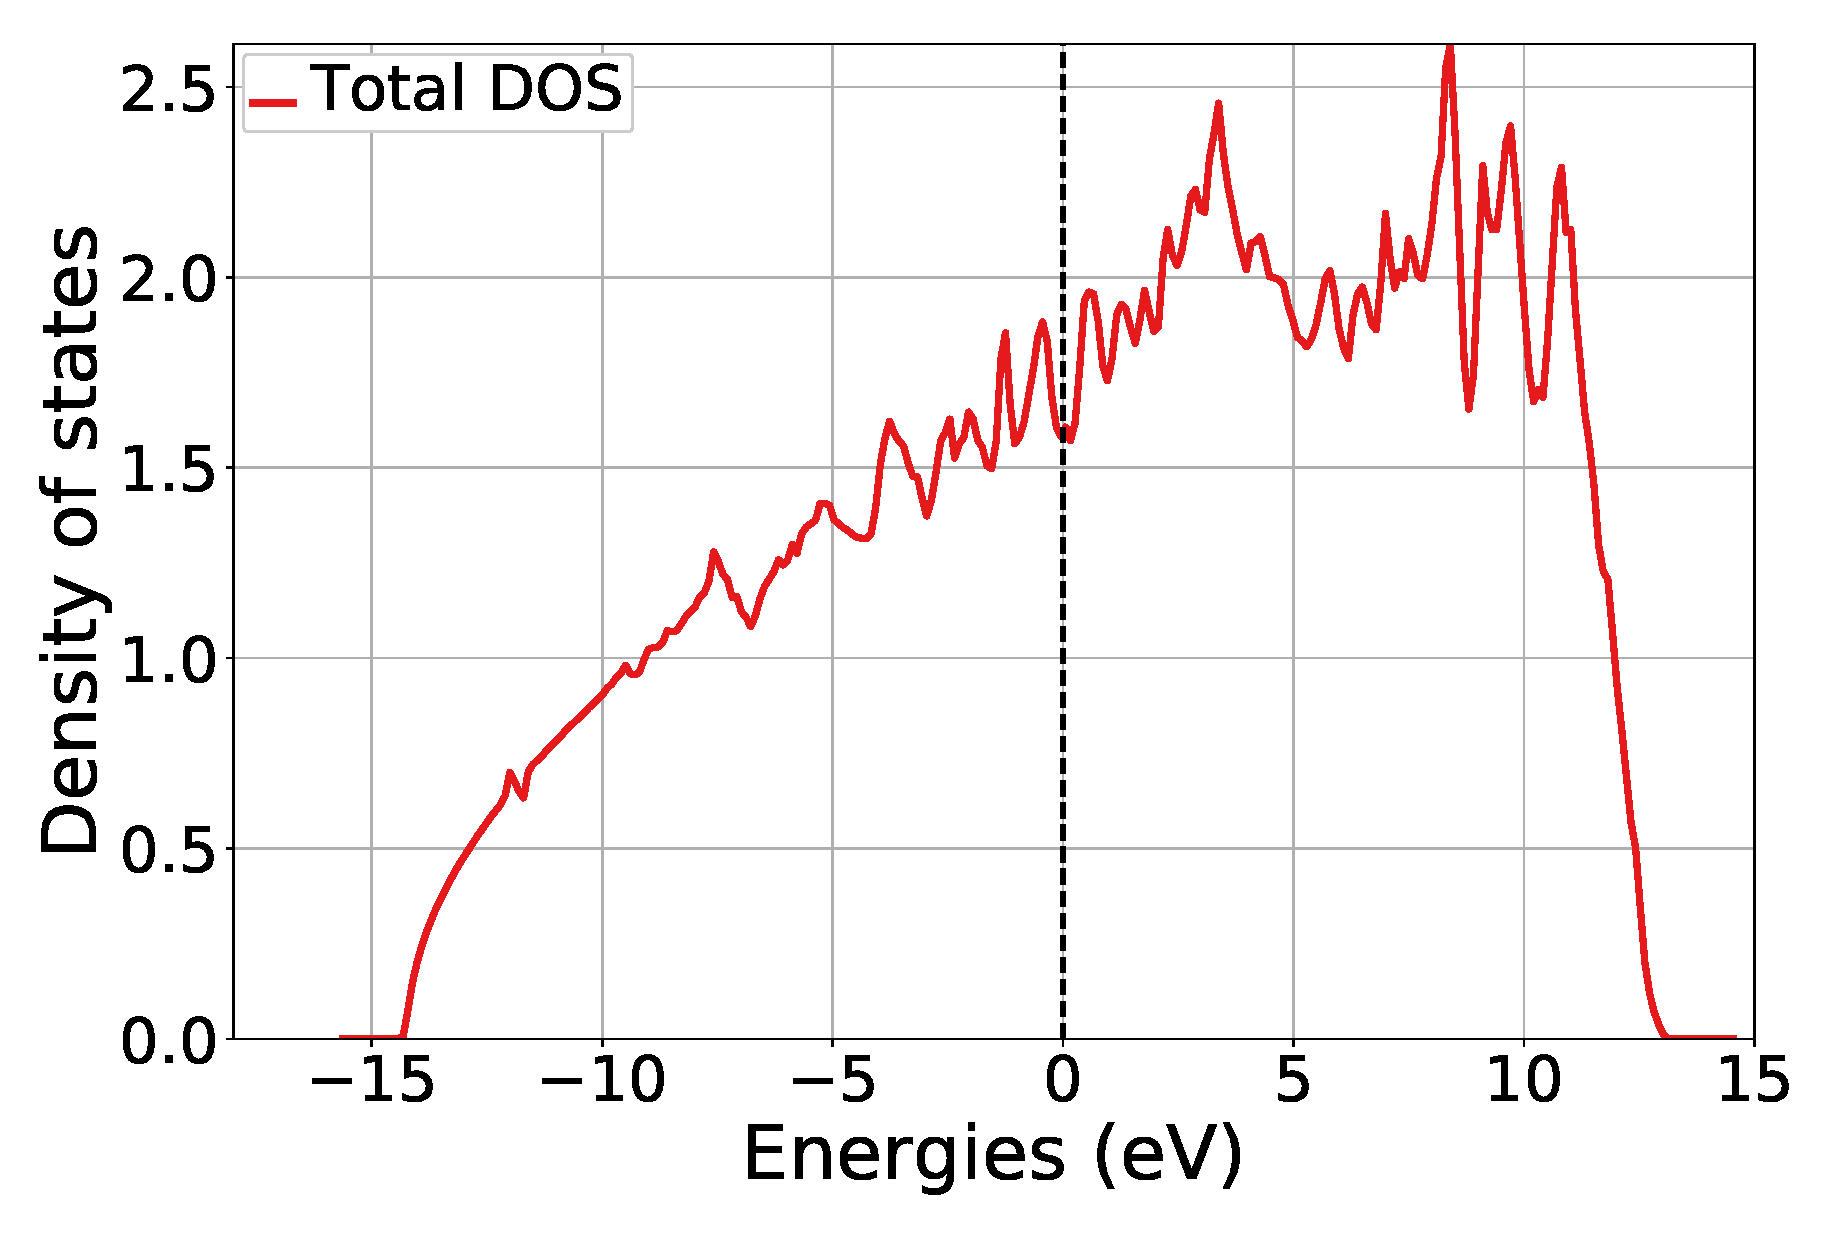
\includegraphics[height=1.5in,width=2.2in,viewport=0 0 890 570,clip]{Figures/VASP_FCC_Si-DOS_4.eps}
%\hspace*{0.01in}
%\includegraphics[height=1.5in,width=2.2in,viewport=0 0 890 570,clip]{Figures/VASP_FCC_Si-DOS_1.eps}
%\caption{\fontsize{7.2pt}{4.2pt}\selectfont{\textrm{The Density of States of FCC-Si from VASP.}}}%
%\label{FCC_Si-DOS}
%\end{figure} 
%\vspace*{-0.2in}
%		\textcolor{blue}{初基原胞(\textrm{primitive cell})用能带表示电子结构:~包含对称性信息}\\
%\vspace*{0.1in}
%		\textcolor{red}{超晶胞(\textrm{super cell})适合用态密度表示电子结构信息}
%}
%

\frame
{
	\frametitle{对称性分析:~空间群对称性}
\begin{minipage}[b]{0.52\linewidth}
	空间群判断模块\textcolor{blue}{\textbf{SGROUP}}:~确定体系所属空间群
	\begin{enumerate}
		\item 通过检查晶胞中许可的平移操作数目,确定最终的点群和空间群的对应关系\\
			{\fontsize{7.2pt}{4.2pt}\selectfont{(32点群-230空间群对应列表)}}
		\item 根据确定的空间群名,输出对应的空间群操作表示矩阵\\{\fontsize{7.2pt}{4.2pt}\selectfont{(点群矩阵+平移矢量)}}
	\end{enumerate}
\end{minipage}
\hfill
\begin{minipage}[b]{0.46\linewidth}
\begin{figure}[h!]
\centering
\vspace*{-0.2in}
\includegraphics[height=3.05in,width=1.55in,viewport=0 50 840 2255,clip]{Figures/VASP_sym-detail.png}
\label{Space_Symmetry}
\end{figure} 
\end{minipage}
}

\frame
{
	\frametitle{成果}
	\begin{itemize}
%		\setlength{\itemsep}{25pt}
		\item 软件著作权\\
			\vskip 5pt
			\fontsize{7.5pt}{4.2pt}\selectfont{晶体对称性分析与电子结构标准化软件\textrm{V1.0}}
\begin{figure}[h!]
	\vspace*{-0.1in}
\centering
\includegraphics[height=2.5in]{Figures/Certificate-2.jpg}
%\caption{\fontsize{6.5pt}{4.2pt}\selectfont{\textrm{MP}型\textrm{La}-六铝酸盐.}}%
\label{Certificates}
\end{figure}
	\end{itemize}
}

\frame
{
	\frametitle{对称性分析:~空间群对称性算例}
	基于\textrm{VASP~}代码开发的空间群分析:~\textrm{HCP-Si}结构对称性分析
\begin{figure}[h!]
\centering
%\vspace*{-0.1in}
\includegraphics[height=2.2in,width=1.9in,viewport=0 0 520 570,clip]{Figures/HCP_Si_Symm-1.png}
\hspace*{0.01in}
\includegraphics[height=2.2in,width=1.9in,viewport=0 0 520 580,clip]{Figures/HCP_Si_Symm-2.png}
\caption{\fontsize{7.2pt}{4.2pt}\selectfont{\textrm{Space-Group-Analysis of HCP-Si developed from VASP codes.}}}
\label{Symmetry_Analysis}
\end{figure} 
}

\frame
{
	\frametitle{对称性分析:~空间群对称性算例}
	基于\textrm{VASP~}代码开发的空间群分析:~\textrm{HCP-Si}结构对称性分析
\begin{figure}[h!]
\centering
\includegraphics[height=2.3in,width=1.9in,viewport=0 0 520 600,clip]{Figures/HCP_Si_Symm-3.png}
\hspace*{0.01in}
\includegraphics[height=2.3in,width=1.1in,viewport=0 0 270 560,clip]{Figures/HCP_Si_Symm-4.png}
\caption{\fontsize{7.2pt}{4.2pt}\selectfont{\textrm{Space-Group and the operating-matrix of HCP-Si.}}}
\label{Space_Group_Analysis}
\end{figure} 
}

%\frame
%{
%	\frametitle{对称性判断与能带路径标准化}
%	\begin{itemize}
%		\item 基于\textrm{VASP~}的对称性分析,标准化$\vec k$\textrm{-path~}路径的自动生成\\(\textcolor{purple}{针对不同\textrm{Bravais~}格子,枚举“标准化”路径的$\vec k$-点分布})
%	\end{itemize}
%\begin{figure}[h!]
%\centering
%\hspace*{-0.18in}
%\subfigure[{\fontsize{6.2pt}{4.2pt}\selectfont{\textrm{Procedure for Point-Group}}}]{
%\label{Procedure_Symmetry}
%\includegraphics[height=2.0in,width=1.85in,viewport=0 0 580 570,clip]{Figures/Procedure_symmetry.png}}
%%\vskip 0.10in
%\subfigure[{\fontsize{6.2pt}{4.2pt}\selectfont{\textrm{Procedure for $\vec k$-path generation}}}]{
%\label{Procedure_sgroup}
%\includegraphics[height=2.0in,width=2.15in,viewport=0 0 670 570,clip]{Figures/Procedure_sgroup.png}}
%\label{Procedure_Symmetry_Sgroup}
%\end{figure}
%}
%
\frame
{
	\frametitle{对称性判断与能带路径标准化}
%	\frametitle{\textrm{VASP~}软件的对称性判断与能带$\vec k$-\textrm{path}}
	应用标准化能带$k$-\textrm{path}计算得到\textrm{FCC-Si}的\textrm{Band}\\{\fontsize{7.3pt}{6.2pt}\selectfont{(算例来源:~\url{http://cms.mpi.univie.ac.at/wiki/index.php/Fcc_Si_bandstructure})}}\\

\begin{figure}[h!]
\centering
\vspace*{-0.1in}
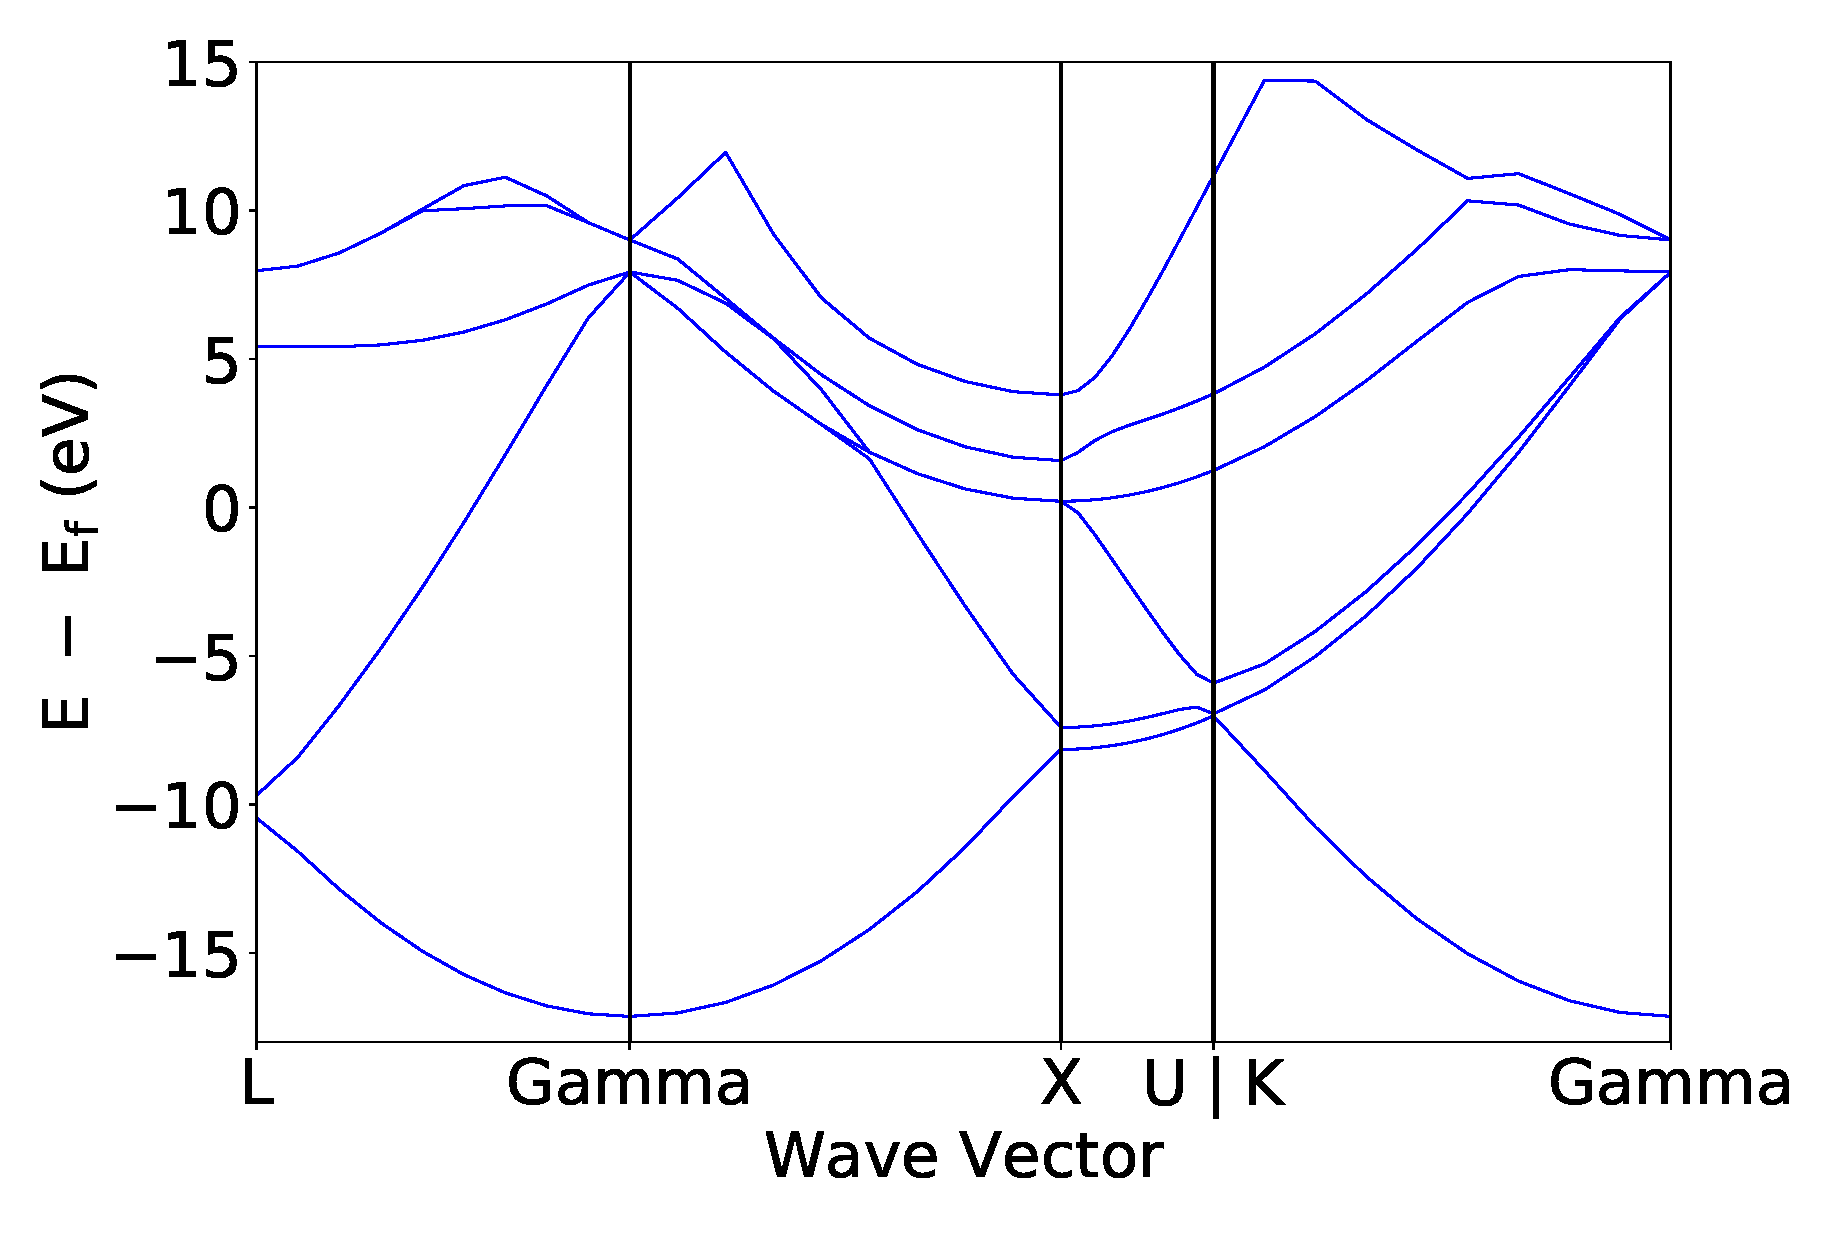
\includegraphics[height=2.0in,width=2.7in,viewport=0 0 890 570,clip]{Figures/FCC_Si-Band_pymatgen.eps}
\hspace*{0.01in}
\includegraphics[height=1.5in,width=1.4in,viewport=280 0 850 600,clip]{Figures/FCC_Si-Brillouin-zone.png}
\caption{\fontsize{7.2pt}{4.2pt}\selectfont{\textrm{The Band-structure of FCC-Si and its standard $\vec k$-path.}}}%
\label{FCC_Si-Band}
\end{figure} 
}

\frame
{
	\frametitle{后续工作:~复杂体系的对称性}
	在\textrm{VASP~}中,$\mathrm{Ni}:\mathrm{Ni}_3\mathrm{Al}$体系的对称性判断,
\begin{figure}[h!]
\centering
%\vspace*{-0.1in}
\includegraphics[height=2.6in,width=3.5in,viewport=0 0 680 530,clip]{Figures/VASP_Alloy_Ni-Al_symmetry.png}
%\caption{\fontsize{7.2pt}{4.2pt}\selectfont{\textrm{Basic database schema for storing periodic crystal structures. Ref\cite{CMS50-2295_2011}}}}%
\label{Alloy_Ni-Al-OUTCAR}
\end{figure} 
}

\frame
{
	\frametitle{后续工作:~复杂体系的对称性}
	\begin{itemize}
   		\setlength{\itemsep}{15pt}
		\item 当前各类软件的对称性判断模块都是在传统的群表示理论基础上开发的,主要适用于理想单晶的对称性判断
		\item 群论基本思想:~利用空间对称元素(平移或滑移、旋转、镜面、反演)约化重复单元中原子间的位置关系,实现对称问题的完备表示\\
			\textcolor{blue}{\textcolor{magenta}{初基原胞(\textrm{primitive cell})}是对称性判断的核心}
%		\item 程序中已经考虑了体系中平移操作的判断,但没有给出确定空间群(\textrm{Space-Group})方案
		\item 针对超晶胞(\textrm{super-cell}),特别是合金体系,\textcolor{red}{有更复杂的需求}
			\begin{itemize}
   				\setlength{\itemsep}{10pt}
				\item \underline{\textcolor{blue}{如何快速地确定\textcolor{magenta}{实际最小重复单元}及其元素组成}}
				\item \textcolor{blue}{\textcolor{magenta}{合金元素的存在}对于对称性判断的影响}
				\item \textcolor{blue}{\textcolor{magenta}{界面}与\textcolor{magenta}{多相合金}对于对称性判断的影响}
			\end{itemize}
	\end{itemize}
}

\section{\rm{VASP}的基态总能量计算与势能零点}
\frame
{
	\frametitle{晶体总能量的一般表示}
基于\textrm{DFT}的晶体总能量$E_T$由晶格中的电子能量$E_{e-e}$与离子实排斥能$E_{N-N}$之和:~
	\begin{displaymath}
		E_T=E_{e-e}+E_{N-N}=T[\rho]+E_{ext}+E_{\mathrm{Coul}}+E_{\mathrm{XC}}+E_{N-N}
	\end{displaymath}
根据\textrm{Kohn-Sham}方程,其中动能泛函用单电子能量表示为
\begin{displaymath}
	T[{\rho}]=\sum_in_i\langle\psi_i|\varepsilon_i-V_{\mathrm{KS}}|\psi_i\rangle
\end{displaymath}
$n_i$是$\psi_i$上的电子占据数,$\varepsilon_i$是其能量本征值,周期体系的总能量表达式在动量空间($\vec K$空间)计算更方便
\begin{displaymath}
	\hspace*{-15.0pt}	E_T=\textcolor{red}{\sum_in_i\varepsilon_i}-\dfrac{\Omega}2\sum_{\textcolor{red}{\vec k\neq 0}}\rho^{\ast}(\vec k)V_{\mathrm{Coul}}(\vec k)+\Omega\sum_{\vec k}\rho^{\ast}(\vec k)[\epsilon_{\mathrm{XC}}(\vec k)-V_{\mathrm{XC}}(\vec k)]+E_{N-N}
\end{displaymath}
}

\frame
{
	\frametitle{发散项的处理}
总能量表达式中存在若干发散项
\begin{itemize}
	\item $E_{N-N}$求和有无穷多项,\textcolor{red}{是发散的}
	\item $V_{\mathrm{Coul}}(\vec k=0)$\textcolor{red}{是发散的}
	\item 用于求解$\varepsilon_i$的$V_{ext}$的\textrm{Fourier}分量在$\vec k=0$\textcolor{red}{也是发散的}
\end{itemize}
上述三项单独都是发散的,但因为整个体系出于电中性,所以这些发散项相互抵消,是一个常数。
\vskip 10pt
克服发散问题的策略:
\begin{itemize}
	\item 求解\textrm{Kohn-Sham}方程时,先将$V_{\mathrm{Coul}}(\vec k=0)$和$V_{ext}(\vec k=0)$同时置为零,相当于\textcolor{red}{将势能作平移,或者说重新定义势能零点}
	\item 在总能量计算中“补偿”这一平移
\end{itemize}
}

\frame
{
	\frametitle{总能量表达式}
\fontsize{6.5pt}{4.2pt}\selectfont{
由此得到的总能量表达式是
\begin{displaymath}
	\begin{aligned}
		E_T=&\sum_i\varepsilon_i-\dfrac{\Omega}2\sum_{\vec k\neq0}\rho^{\ast}(\vec k)V_{\mathrm{Coul}}(\vec k)\\
		&+\Omega\sum_{\vec k}\rho^{\ast}(\vec k)[\epsilon_{\mathrm{XC}}(\vec k)-V_{\mathrm{XC}}(\vec k)]\\
		&+\sum_s\alpha_s\sum_sZ_s+E_{\mathrm{Ewald}}
	\end{aligned}
\end{displaymath}
}
\begin{figure}[h!]
\centering
\vspace*{-0.18in}
\includegraphics[height=1.85in,width=2.2in,viewport=0 0 600 495,clip]{Figures/VASP_Total_ENE.png}
\caption{\small \textrm{The Total-E calculated by VASP.}}%(与文献\cite{EPJB33-47_2003}图1对比)
\label{TOTEN_VASP}
\end{figure}
}

\section{\rm{VASP}软件的特色与并行}
\frame
{
	\frametitle{\textrm{VASP}计算的特色}
		疫情期间,对\textrm{VASP}代码作了系统的梳理和解读,总体把握了\textrm{VASP}计算实现的技术核心
	\begin{itemize}
		\item \textrm{VASP}很好地平衡了计算效率和精度的问题,主要通过几个方面保证计算的高效能
	\begin{enumerate}
	     \item 迭代与优化算法的多样性\\
		     将电荷密度迭代 \textrm{\&\&}和体系总能量优化划归为类似的数值优化问题,采用多种优化算法,包括:\\
			\textcolor{blue}{\textrm{Pseudo-Newton、Conjugate-Gradient、Broyden~mix、damping-factor、RMM-DIIS}}
	     \item 计算过程中,尽可能使用局域基(原子轨道基)函数:~\\
		     优化的投影函数也尽可能在实空间表示,大大节约了基组的维度
	     \item \textrm{PAW}原子数据集:\textcolor{blue}{优异的赝势}确保计算精度
	     \item \textrm{FFT}变换的网格分配:~\textrm{FFT}网格与并行节点数目实现自动均衡匹配,有效提升并行效率
	\end{enumerate}
	\end{itemize}
}

\frame
{
	\frametitle{\textrm{VASP}计算的并行实现}
	\begin{itemize}
	     \item 中间层的设计思想:~并行计算中\textrm{FFT}网格、实空间基函数与计算节点的匹配\\
		     \textcolor{magenta}{通过子程序\textrm{mgrid.F}生成中间层,建立映射关系,实现并行负载与计算节点分配的匹配,降低\textrm{FFT}变换和实空间并行的节点间通信,提升并行效率}
\begin{figure}[h!]
	\vspace{-0.10in}
\centering
%\includegraphics[height=2.7in,width=4.0in,viewport=0 0 1180 875,clip]{Figures/dual_grid.png}
\includegraphics[height=0.8in,width=3.2in,viewport=0 0 1500 450,clip]{Figures/VASP_FFT-MPI_Reciprocal.png}
\vskip 0.5pt
\includegraphics[height=0.6in,width=3.4in,viewport=0 0 730 150,clip]{Figures/VASP_FFT-MPI_Real.png}
\caption{\tiny \textrm{VASP:~ Reciprocal-Real space layout for grids in MPI.}}%(与文献\cite{EPJB33-47_2003}图1对比)
\label{MPI-FFT}
\end{figure} 
	\end{itemize}
}

%\appendix
%------------------------------------------------------------------------Reference----------------------------------------------------------------------------------------------
%\begin{thebibliography}{99}
%-----------------------------------------------------------------------------------------------------------------------------------------------------------------------%
%\frame
%{
%\frametitle{主要参考文献}
%{\small
%\bibitem{Singh_Book}\textrm{D. J. Singh. \textit{Plane Wave, PseudoPotential and the LAPW method} (Kluwer Academic, Boston,USA, 1994)}					%
%  \nocite{*}																				%
%}
%}
%\end{thebibliography}
%\begin{thebibliography}
%\frame
%{
%\frametitle{主要参考文献}
%\bibliography{Ref_2020-11-28}%
%\bibliographystyle{../ref/mybib}%
%\nocite*{}
%}
%\end{thebibliography}
%{\small
%\phantomsection\addcontentsline{toc}{section}{Bibliography}	 %直接调用\addcontentsline命令可能导致超链指向不准确,一般需要在之前调用一次\phantomsection命令加以修正	%
%\bibliography{Myref}																			%
%\bibliographystyle{mybib}																		%
%  \nocite{*}																				%
%}
%-----------------------------------------------------------------------------------------------------------------------------------------------------------------------%


%-----------------------------------------------------------Beamer下不建议使用bib,因为涉及分页--------------------------------------------------------------------------%
%{\small
%\phantomsection\addcontentsline{toc}{section}{Bibliography}	 %直接调用\addcontentsline命令可能导致超链指向不准确,一般需要在之前调用一次\phantomsection命令加以修正	%
%\bibliography{Myref}																			%
%\bibliographystyle{mybib}																		%
%  \nocite{*}																				%
%}

%------------------------------------------------------------------------------------------------------------------------------------------------------------------------------%

%-------------------------------------------------------------------------Thanks------------------------------------------------------------------------------------------------
%\section{致谢}
%\frame
%{
%\frametitle{致$\quad$谢}
%\begin{itemize}
%    \setlength{\itemsep}{20pt}
%  \item 感谢本团队高兴誉、吴泉生、宋红州等各位老师参与的讨论
%  \item 感谢莫所长、宋主任以及软件中心各位老师和同事
%  \item 感谢王崇愚先生的帮助
%\end{itemize}
%}

\logo{}									%不显示logo
\frame
{
\vskip 60 pt
%%\hskip 10pt \textcolor{blue}{\Huge 感谢答辩委员会各位老师\,\textrm{!}}\\
%\vskip 35 pt
\hskip 60pt \textcolor{blue}{\Huge 谢谢大家\:!}
%%\vskip 15 pt
%%\hskip 40pt \textcolor{blue}{\Huge \textrm{for your attention\:!}}
}

%-------------------------------------------------------------------------------------------------------------------------------------------------------------------------------

\clearpage
%\end{CJK*}
\end{document}
